\chapter{Related Works}
\label{sec:related-works}

Both windowing systems and 3D user interfaces have received a great deal of research over the past few decades, and these fields intersect in a number of ways, so placing this thesis within existing research is somewhat complicated. 

The system described in this paper has the key design goal of being able to seamlessly handle both 2D and 3D interface contexts in the same 3D interface space, so we will compare it to existing research based on this. This primary design goal can be broken down into several secondary goals, including allowing applications to request 2D and 3D windows in the same manner, allowing users to interact with 2D and 3D windows in the same manner, and allowing applications to receive 2D and 3D input in the same manner. Other design goals include allowing applications to use the windowing system without needing to be started by it and allowing 2D applications to window into the 3D space without needing to be modified. To the author's knowledge this set of requirements is not met by any system in existing research.

\section{Two Dimensional Windows in Three Dimensional Environments}
A fair amount of work has been done on managing traditional 2D windows in a 3D space, both in research and, more recently, in production software. These systems can handle multiple 2D windows in a 3D space and can draw the 2D output of a 3D application as a 2D window, but none of them provide a mechanism for unifying the application space with the windowing space for seamless 3D interaction between multiple applications in a single 3D space.

\begin{figure}[ht!]
\centering
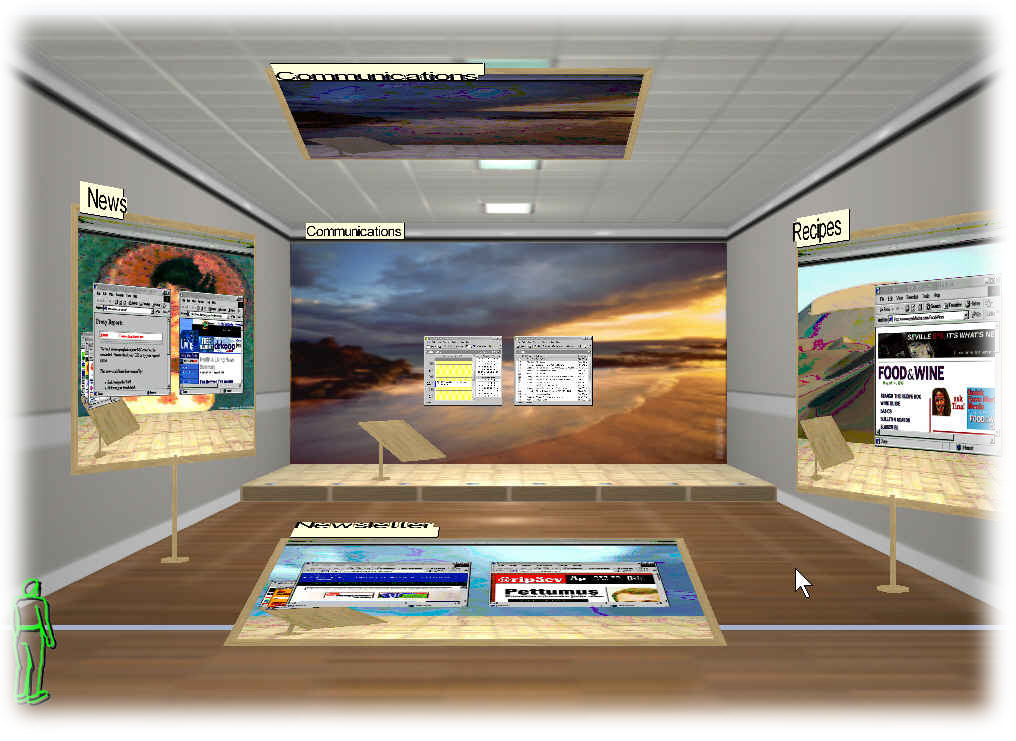
\includegraphics[width=1.0\textwidth]{images/task_gallery.jpg}
\caption{The Task Gallery \protect\cite{task_gallery}}
\end{figure}

The Task Gallery \cite{task_gallery} is a 3D window manager for Microsoft Windows which embeds groups of related windows called 'tasks' into a 3D space to make them appear like artwork hung in a gallery, with the active task on a center 'stage'. This system has some truly 3D user interface elements, like the gallery and the stage, but it exclusively supports 2D windows. 

%\begin{figure}[ht!]
%\centering
%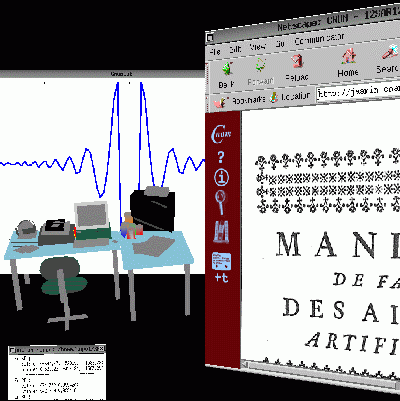
\includegraphics[width=0.5\textwidth]{images/xwindow-immersion.png}
%\caption{Immersion of XWindow applications into a 3D workbench \protect\cite{xwindow_immersion}}
%\end{figure}

Topol describes a system for embedding standard X11 windows into a 3D workspace using techniques similar to those used by modern compositing window managers \cite{xwindow_immersion}. However, like The Task Gallery, this system supports only flat, 2D windows. Additionally, it does not appear that this system support mapping input from the 3D workbench space into the 2D window space.

\begin{figure}[ht!]
\centering
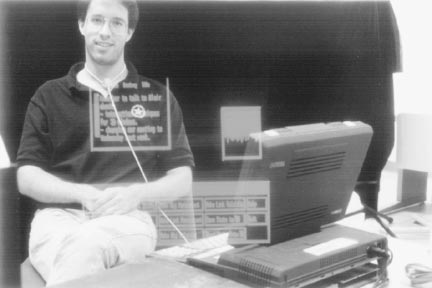
\includegraphics[width=1.0\textwidth]{images/wotw.png}
\caption{Windows on the World \protect\cite{wotw}}
\end{figure}

Feiner et al. demonstrate a similar 3D window management system in an augmented reality setting with their Windows on the World system \cite{wotw}. This system uses a very large X bitmap which applications draw into using traditional means. The display server displays a small portion of this bitmap at a time on a see through head mounted display, and determines which portion of the bitmap to draw into by mapping the pitch and yaw of the user's head onto the x and y coordinates of the bitmap, thereby mapping the bitmap onto a portion of a spherical surface surrounding the users head. Windows can be moved within the bitmap such that they always track the projection of a real world object onto the spherical surface, thereby creating the illusion that the window is attached to that object.
 
\subsection{In Production Software}

As GPU accelerated window compositing has become widely available on consumer hardware (following improved OpenGl support in X.org around 2006) the ability to handle windows in 3D has become broadly available in consumer software.  Some widely used compositing window managers, like Compiz \cite{compiz}, draw window output as textures on 2D surfaces in 3D, allowing them to create compelling 3D visual effects and animate window transitions in 3D space. However, because the architecture of X11 does not give the compositor control of the input system, X11 compositing window managers like Compiz are unable to properly redirect input to the windows while their output is transformed to appear 3D, which seriously limits ability X compositors to create useful 3D interfaces.

\begin{figure}[ht!]
\centering
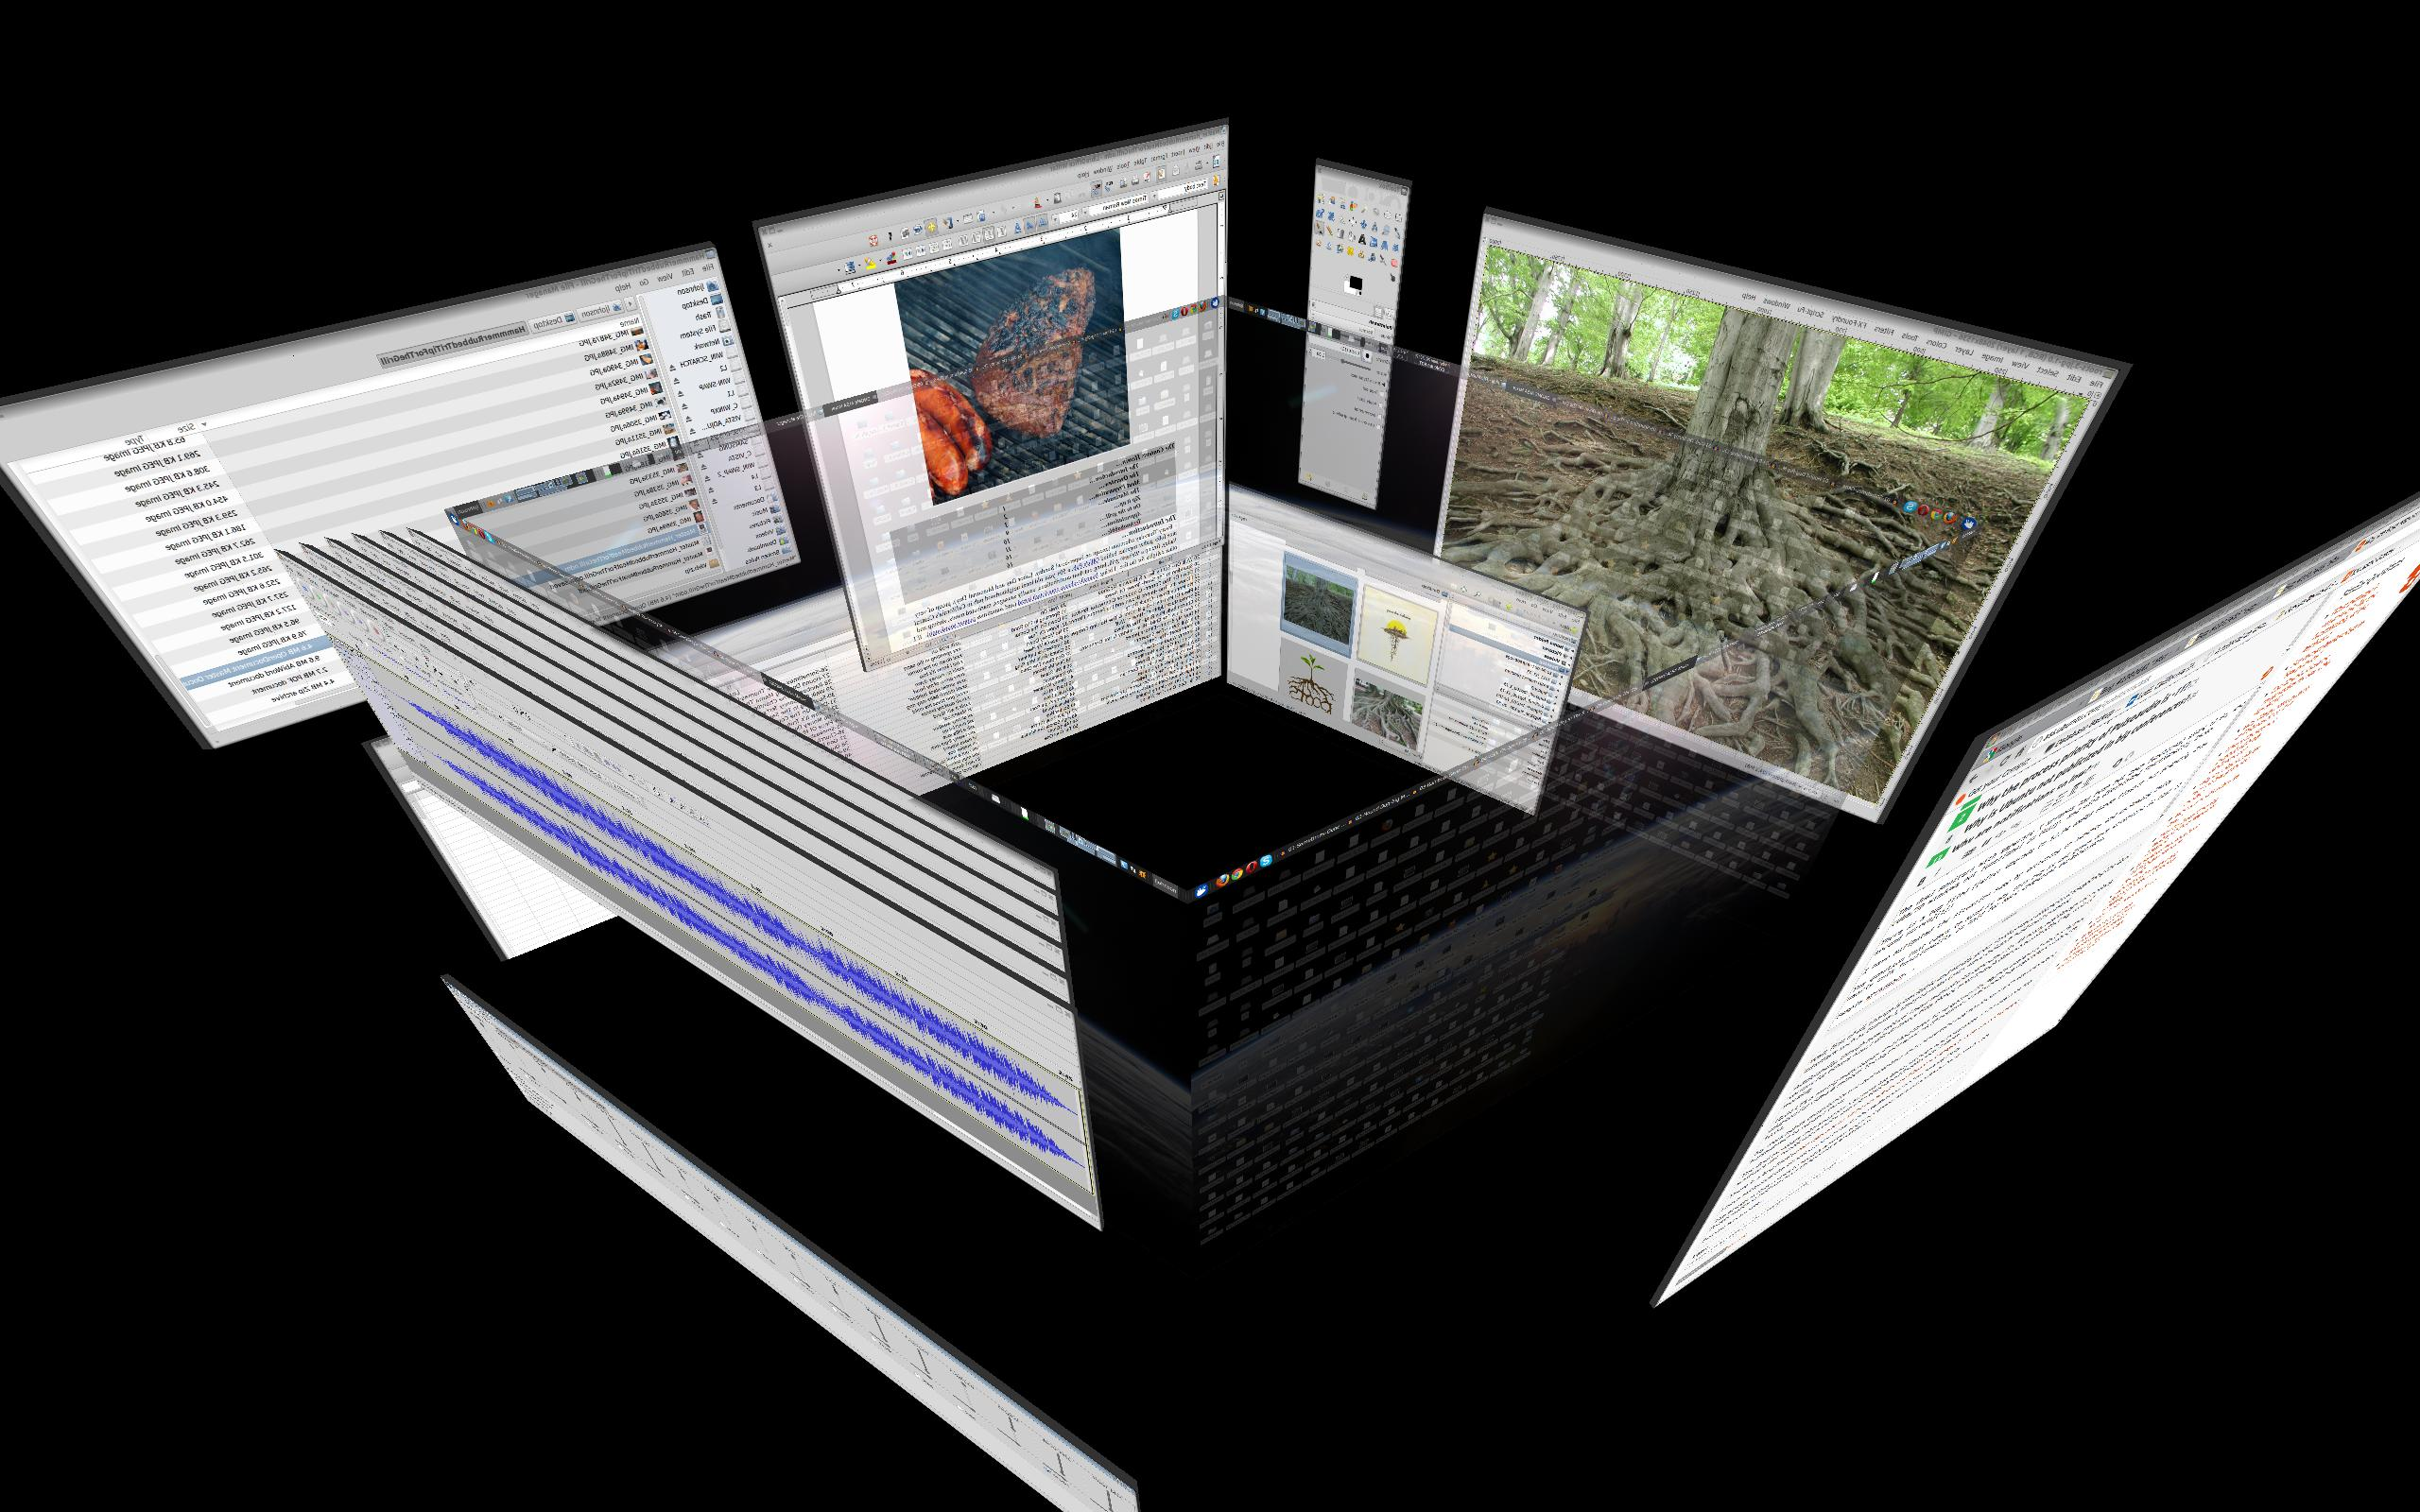
\includegraphics[width=1.0\textwidth]{images/compiz.jpg}
\caption{Compiz Desktop Cube \protect\cite{compiz}}
\end{figure}

The open source community has been seeking to address many of the problems and shortcomings of X11 with the development of a completely new display server protocol called Wayland \cite{wayland}. One of the key differences between Wayland and X is that the display server and the compositor are the same entity, meaning that the compositor can both transform window output to appear embedded in a 3D space while also mapping 3D input back into the 2D window space, allowing traditional 2D windows to be first class citizens of new 3D user interfaces. This, coupled with the simplified architecture of Wayland, is the reason why Wayland forms the basis of the windowing system presented in this thesis.

There are other production windowing systems which allow output from windows to be transformed to appear 3D, used mainly to provide 3D window transition effects like Flip 3D in Windows Vista and Windows 7. To the author's knowledge no production window manager allows normal window interaction while the windows' output is transformed to appear 3D.

\section{Three Dimensional Windows}

There are systems in existing research which explore concepts similar to the 3D windows described in this paper. For the most part what separates them from the work in this thesis is lack of support for windowing by external applications, limitations on what clients are allowed to draw within their windowing volumes, or lack of first class support for 2D windows.

\begin{figure}[ht!]
\centering
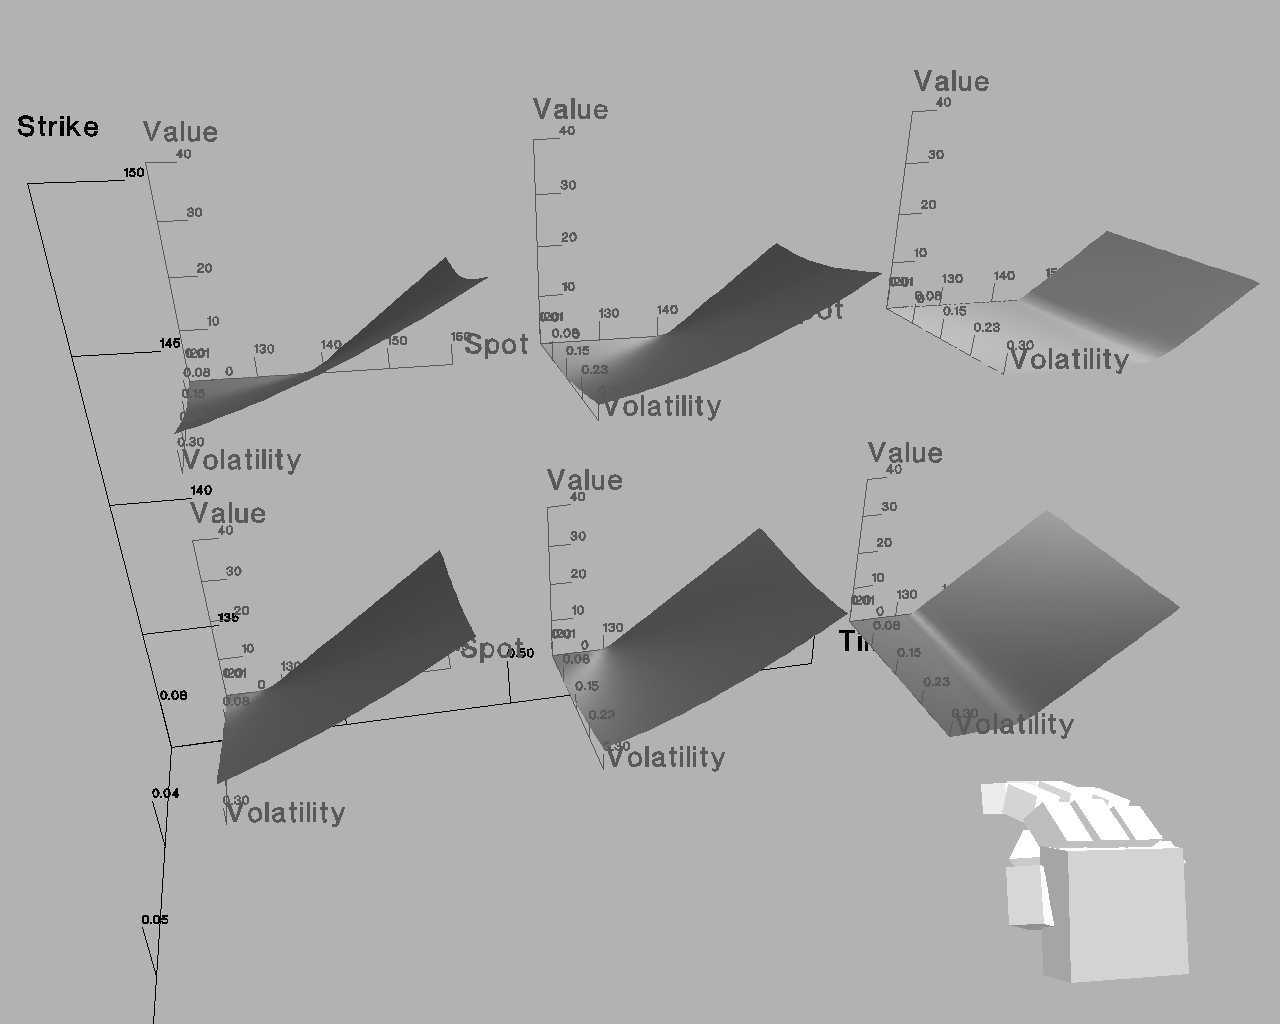
\includegraphics[width=1.0\textwidth]{images/n-vision.png}
\caption{The n-Vision Test Bed \protect\cite{nvision}}
\end{figure}

The earliest work (to the author's knowledge) which explores such a concept is Feiner and Besher's n-Vision testbed \cite{nvision} in 1990, a system designed to facilitate the visualization of high dimensional data using a hierarchy of nested 3D visualization volumes called 'boxes'. Each box draws a 3D slice of the multidimensional space by mapping the high dimensional function across 2 selected independent variables within the box, with all other independent variables held fixed within the box at a value determined by the box's position within its parent box. This nested hierarchy of boxes is much like a 3D analogue of the X protocol's hierarchy of 2D rectilinear windows (as the authors note), but it is not designed to allow third party applications to create such volumes and draw content inside of them. It also lacks support for 2D windows, and the capabilities of the system appear to be limited to graphing multivariate functions.

\begin{figure}[ht!]
\centering
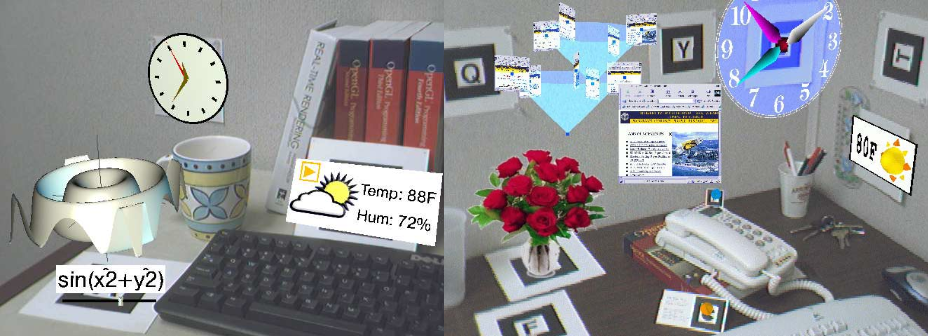
\includegraphics[width=1.0\textwidth]{images/arwin.png}
\caption{Example ARWin Desktops \protect\cite{anywhere-augmentation}\protect\cite{arwin}. Note the function graph and bouquet programs, which draw 3D content into the 3D interface space.}
\end{figure}

DiVerdi demonstrates a 3D augmented reality window manager called ARWin \cite{arwin} which he uses to manage 3D user interface elements and 2D windows in his Anywhere Augmentation system \cite{anywhere-augmentation}. It is difficult to firmly compare this thesis to ARWin because the description of ARWin does not go into great detail about the system's implementation. One difference that is clear is that the system lacks native support for 2D windows, instead supporting 2D windows through a VNC client which outputs the windows content to a texture (which limits 2D support to applications without hard latency requirements). While their system supports multiple applications drawing 3D user interface elements in the same 3D space, it is not clear what constraints are imposed on this process or the mechanism by which 3D applications draw content in the 3D space. It is also unclear how applications request a session with the display manager, and even if this is possible without the display manager starting the application itself. No documentation regarding the windowing mechanism could be found. 

\section{The Three Dimensional Workspace Manager (3DWM)}

The system in existing research which appears to be the closest thing to the system described in this thesis is 3DWM \cite{3dwm}, a system designed to provide a network transparent hardware abstraction layer for 3D user interfaces and a reusable 3DUI toolkit to ease the development and research of new 3D user interfaces. Like the system described in this thesis (and like the X Window Protocol and the Wayland display server protocol) the basic system architecture consists of a display server which manages the input and output hardware, and a set of independent client applications which are able to request that the display server notify them of input events and draw content for them on the output hardware. 

\begin{figure}[ht!]
\centering
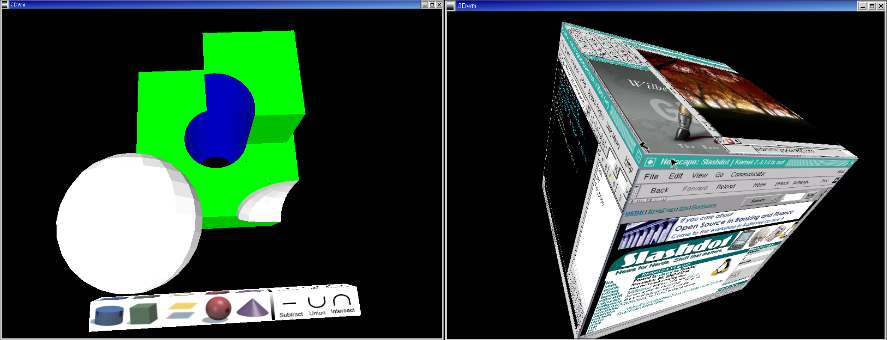
\includegraphics[width=1.0\textwidth]{images/3dwm.png}
\caption{The Three Dimensional Workspace Manager \protect\cite{3dwm}. On the left is a constructive solid geometry modeller, demonstrating the support for 3D applications. On the left we see it texturing multiple X11 desktops (over VNC) onto a 3D cube.}
\end{figure}

Unlike the system described here, but much like early uses of X, their display server draws user interface primitives on the behalf of the client and does not allow the clients to directly control the way the primitives are drawn. This is done because (like early X) network transparency was one of their core design goals, and transmission of pixel buffers from real-time graphics applications to the display server requires much greater bandwidth and much lower latency than most networks are able to provide. The system described in this thesis avoids this (by sacrificing network transparency) because although it gives the system a unified look and feel, it requires that applications perform many transactions with the display server in order to accomplish basic user interface tasks and limits the behaviour and appearance of application user interfaces to functionality supported by the display server. These are the same factors which led to the abandonment of the widespread use of X11's primitive drawing capability and the loss of its pure network transparency (through the use of direct rendering extensions to X) and are two of the major factors motivating the development of Wayland as a replacement for X. 

3DWM does support multiple application contexts in a single 3D space, and allows applications to request volumes for their personal use, which is very similar to the concept of 3D windows presented in this thesis (and is compared to the concept of windows by the authors). However, unlike traditional windows, and unlike the 3D windows presented in this thesis, client applications do not have full control of what is drawn inside of their windowing context. Instead, clients are only able to request that the display server draw primitives inside of their volume, and if the primitives the display server provides do not meet the needs of the application then the developers have no choice but to modify the display server.

Another shortcoming of 3DWM is the lack of native support for 2D windows inside the 3D application space. While the need to support 2D applications is not ignored completely, it is viewed as 'legacy' support during a 'transitionary phase' to completely 3D interfaces and as such 2D applications are not treated as first class clients of the display server. Instead, they implement a custom VNC client which writes a remote desktop into a texture which the display server then applies to a surface in the 3D space. While this does indeed provide simultaneous support for 2D applications running on many platforms, it does not allow individual 2D and 3D applications to be mixed and used together in the same 3D space. 
